
\begin{frame}{} \small
\vskip1em
\begin{minipage}{.56\textwidth} 
\colorbox{gray}{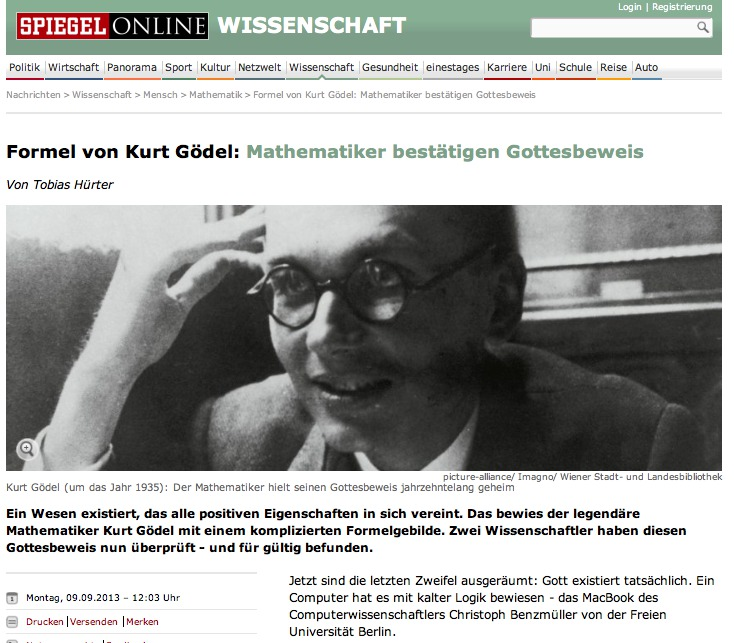
\includegraphics[width=\textwidth]{Images/News/spiegel1}} 
\vskip1em
Germany \\
- Telepolis \& Heise \\
- Spiegel Online \\
- FAZ \\
- Die Welt \\
- Berliner Morgenpost \\
- Hamburger Abendpost \\
- \ldots \\
\end{minipage} \hfill
%
\begin{minipage}{.3\textwidth}
Austria \\
- Die Presse \\
- Wiener Zeitung \\
- ORF \\
- \ldots \\

Italy \\
- Repubblica \\
- Ilsussidario \\
- \ldots \\

% Russia \\
% - \ldots \\

India \\
- DNA India \\
- Delhi Daily News \\
- India Today \\
- \ldots \\

US \\
- ABC News \\
- \ldots \\

International \\
- Spiegel International \\
- Yahoo Finance \\
% - CNET \\
- United Press Intl. \\
- \ldots \\
\end{minipage}
\end{frame}

\begin{frame}{Introduction --- Quick answers to your most pressing questions!} \large
\colorbox{gray}{
\includegraphics[width=\textwidth]{Images/News/MacBookGrab}} 
\pause
\vfill
Are we in contact with Steve Jobs? \hfill No \\[2em]
Do you really need a MacBook to obtain the results? \hfill No \\[2em]
Is Apple sending us money? \hfill No \\
\, \hfill (but maybe they should)
\end{frame}

\begin{frame}{Introduction}\large
%Ontological argument: Conclude that God exists from premises by pure, a priori reasoning.
\begin{block}{Def: \textcolor{blue}{Ontological Argument/Proof}}
* deductive argument \\

* for the existence of God \\

* starting from premises, which are justified by pure reasoning,
i.e. they do not depend on observation of the world.
\end{block}

\vfill \pause
Existence of God: different types of arguments/proofs\\[.2em]
\begin{itemize}
\item[---]a posteriori (use experience/observation in the world)
  \begin{itemize}
  \item[------]teleological
  \item[------]cosmological
  \item[------]moral
  \item[------] \ldots
  \end{itemize}  
\item[---]a priori (based on pure reasoning, independent)
  \begin{itemize}
  \item[------]\textcolor{blue}{ontological argument}
    \begin{itemize}
    \item[------]definitional 
    \item[------]modal 
    \item[------] \ldots
    \end{itemize}
  \item[------]other a priori arguments
  \end{itemize}
\end{itemize}
\end{frame}

\begin{frame}{Introduction}
\vskip1em
\emph{\huge Wohl eine jede Philosophie kreist um den ontologischen
  Gottesbeweis} \\[1.5em]
(Adorno, Th. W.: Negative Dialektik. Frankfurt a. M. 1966, p.378)
\vfill
\begin{center}
\fcolorbox{gray}{white}{
\begin{minipage}{.9\textwidth}
\ldots \hfill
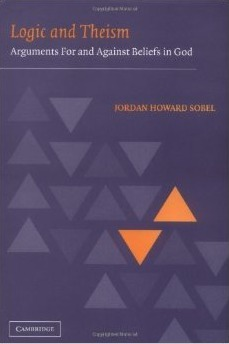
\includegraphics[height=2cm]{Images/Books/buch3.jpg} \hfill

\includegraphics[height=2cm]{Images/Books/buch2.jpg} \hfill 
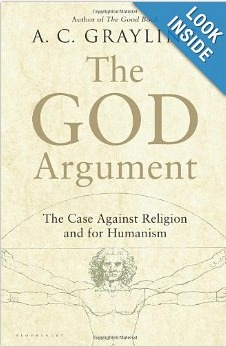
\includegraphics[height=2cm]{Images/Books/buch4.jpg} \hfill
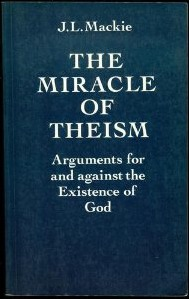
\includegraphics[height=2cm]{Images/Books/buch5.jpg} \hfill
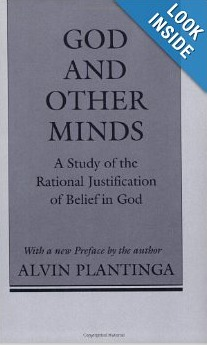
\includegraphics[height=2cm]{Images/Books/buch6.jpg} \hfill

\includegraphics[height=2cm]{Images/Books/buch1.jpg} \hfill
\ldots
\end{minipage}
}
\end{center}
\end{frame}


\begin{frame}{Introduction} \Large
{Rich history on ontological arguments (\textcolor{blue}{pros} and \textcolor{red}{cons})}\\[1em]

\hskip-.5em
\ldots\rotatebox[origin = bl,width = 0mm]{65}{\textcolor{blue}{Anselm v. C.}} \hskip-2.3em
          \rotatebox[origin = bl]{65}{\textcolor{red}{Gaunilo}} \hskip-1.3em
\ldots  \rotatebox[origin = bl]{65}{\textcolor{red}{Th. Aquinas}}  \hskip-2.3em
\ldots\ldots   \rotatebox[origin = bl]{65}{\textcolor{blue}{Descartes}} \hskip-1.7em
               \rotatebox[origin = bl]{65}{\textcolor{blue}{Spinoza}} \hskip-1.3em
               \rotatebox[origin = bl]{65}{\textcolor{blue}{Leibniz}}  \hskip-1.2em
\ldots  \rotatebox[origin = bl]{65}{\textcolor{red}{Hume}}  \hskip-1em
          \rotatebox[origin = bl]{65}{\textcolor{red}{Kant}}  \hskip-.8em
\ldots  \rotatebox[origin = bl]{65}{\textcolor{blue}{Hegel}}  \hskip-1.3em
\ldots  \rotatebox[origin = bl]{65}{\textcolor{red}{Frege}}  \hskip-1.3em
\ldots  \rotatebox[origin = bl]{65}{\textcolor{blue}{Hartshorne}} \hskip-1.9em
          \rotatebox[origin = bl]{65}{\textcolor{blue}{Malcolm}}  \hskip-1.4em
          \rotatebox[origin = bl]{65}{\textcolor{red}{Lewis}}  \hskip-1em
          \rotatebox[origin = bl]{65}{\textcolor{blue}{Plantinga}}  \hskip-1.6em
          \rotatebox[origin = bl]{65}{\textcolor{blue}{G\"odel}}   \hskip-1.2em
\ldots \\[1em]

\pause
\vfill
Anselm's notion of God:\\
\,\hfill \emph{``God is that, than which nothing greater can be
  conceived.''} \\[1em]

G\"odel's notion of God:\\
\,\hfill \emph{``A God-like being possesses all `positive' properties.''} \\[1em]

To show by logical reasoning: \\
\,\hfill \emph{``(Necessarily) God exists.''} \\[1em]

% \rnode{n2}{}\emph{}
% \ncline[nodesep=2pt,linecolor=black,linewidth=1pt]{->}{n1}{n2}
\end{frame}


\begin{frame}{Introduction} \Large
Different Interests in Ontological Arguments: \\[1em]
\begin{itemize}
\item \textcolor{blue}{Philosophical:} Boundaries of Metaphysics \& Epistemology
  \begin{itemize}
  \item We talk about a metaphysical concept (God), 
  \item but we want to draw
      a conclusion for the real world. \\[1em]
  \item Necessary Existence (NE): metaphysical NE vs. logical NE  vs. modal NE \\[2em]
  \end{itemize} 
\item \textcolor{blue}{Theistic:} Successful argument should convince atheists \\[2em]
\item \textcolor{red}{Ours:} Can computers (theorem provers) be used \ldots
  \begin{itemize}
  \item \ldots to formalize the definitions, axioms and theorems?
  \item \ldots to verify the arguments step-by-step?
  \item \ldots to fully automate (sub-)arguments? \\[1em]
  \end{itemize}
  \textcolor{red}{\emph{``Computer-assisted Theoretical Philosophy''}}
\end{itemize}
\end{frame}

\begin{frame}{Introduction} \large
\hskip-1em Challenge: \hfill No provers for \emph{Higher-order Quantified Modal Logic\/} (\textcolor{red}{QML}) \\[1em]

\hskip-1em Our solution: \hfill Embedding in \emph{Higher-order Classical Logic\/} (\textcolor{blue}{HOL}) \\
\,\hfill {\small [Benzm\"ullerPaulson, Logica Universalis, 2013]} \\[2em]

\hskip-1em What we did \textcolor{blue}{(rough outline for remaining
  presentation!)}: \\

\begin{itemize}
\item[A:] Pen and paper: \hfill detailed natural deduction proof 
\item[B:] Formalization: \hfill in classical higher-order logic (\textcolor{blue}{HOL})
\item[] Automation: \hfill theorem provers \textsc{Leo-II} and \textsc{Satallax} 
\item[] Consistency: \hfill model finder \textsc{Nitpick (Nitrox)} 
\item[C:] Step-by-step verification: \hfill proof assistant \textsc{Coq} 
\item[D:] Automation \& verification: \hfill proof assistant \textsc{Isabelle} \\[2em]
%\item[ ] Conclusion \\[2em]
\end{itemize}
\hskip-1em  Did we get any new results? \hfill  \textcolor{red}{Yes --- let's discuss this later!}
\end{frame}
